\documentclass{article}
\usepackage{amsfonts}
\usepackage{MnSymbol}
\usepackage{graphicx}
\usepackage{comment}
\title{MVE200 - Läsvecka 2}
\author{Krysset}
\begin{document}
    \tableofcontents
    \clearpage
    \section{Aritmetisk talföljd}
        En aritmetisk talföljd är en talföljd 
        $ a_{1}, a_{2}, a_{3}, ..., a_{n} $ där 
        $ a_{2}-a_{1} = a_{3} - a_{2} = a_{4} - a_{3} = ... = a_{n} - a_{n-1} $\\
        {\bf Ex:}\\
        \indent 1,2,3...,100 Skillnaden är 1\\
        \indent 3,7,11,15,19,... Skillnaden är 4\\
        Om $ a_{1}, a_{2}, ..., a_{n} $ är en aritmetisk talföljd så kallas 
        $ a_{1}, a_{2}, ..., a_{n} = \sum_{i = 1}^{n} ai$ för en aritmetisk summa. 
        För en aritmetisk summa gäller $ \sum_{i = 1}^{n} ai = n \cdot \frac{a_{1} \cdot a_{n}}{2} $ 
        där n är antalet termer.\\
        En talföljd $ a_{1}, a_{2}, ..., a_{n} $ kallas geometrisk om 
        $ \frac{a_{2}}{a_{1}} = \frac{a_{3}}{a_{2}} = ... = \frac{a_{n}}{a_{n-1}} $ \\
        {\bf Ex:}\\
        \indent $2,4,8,16,32$ Kvoten är 2\\
        \indent $4,12,36,108$ Kvoten är 3\\
        \\
        Om $a_{1},..., a_{n} $ är geometrisk kallas $ \sum_{i = 1}^{n} ai $ för en geometrisk summa.\\
        Om $ C = \frac{a_{2}}{a_{1}} = ... = \frac{a_{n}}{a_{n-1}} $ och $ c \neq 1 $ så är $ \sum_{i = 1}^{n} ai = a_{1} \cdot \frac{c^{n}-1}{c-1} $\\
        \subsection*{Varför?}
            $ a_{1}, a_{2} = a_{1}c, a_{3} = a_{1}c^{2}, ..., a_{n} = a_{1}c^{n-1} $ så 
            $ (c-1) \sum_{i = 1}^{n} ai = (c-1) (a_{1} + a_{1}c + a_{1}c^{2} +... + a_{1}c^{n-1})=
            a_{1}(c-1)(1+c+c^{2}+...+c^{n-1})=
            a_{1}(-1+c-c+c^{2}-c^{2}+...-...-c^{n-1}+c^{n})=
            a_{1}(c^{n}-1) $
    \clearpage
    \section{Induktion och Rekursion}
        \begin{itemize}
            \item Rekursion är en definitionsteknik där man definierar en funktion\/talföljd\/etc "steg för steg"
            \item Induktion är en bevisteknik där man bevisar en följd $ P_{1}, P_{2}, ... $ av utsagor steg för steg
        \end{itemize}
        {\bf OBS!} En oändlig taföljd $ a_{1}, a_{2}, ... $ är samma sak som en funktion $ f:\mathbb{Z}_{+} \rightarrow \mathbb{R} $\\
        "Def" (4.7 i boken)\\
        $ f:\mathbb{Z}_{+} \rightarrow \mathbb{R} $ är en rekursivt definierad om $ \exists a\in \mathbb{Z}_{+} $ så att 
        \begin{enumerate}
            \item f(1), ..., f(a) är givna ("startvärden")
            \item $ \forall n\geq a+1$ är f(n) en funktion av $ f(1), ..., f(n-1) $. ("rekursion") (Dålig förklaring...)
        \end{enumerate}
        INTE BRA!!! 2) är inte tillräckligt precis\\
        Problement i 2):
        \begin{itemize}
            \item Kan jag använda olika funktioner för olika n?
            \item Ser nästan ut så eftersom aantalet argument växer
            \item Vilken typ av funktion får det vara?
        \end{itemize}
        \underline{{\bf Def}}\\
        $ f:\mathbb{Z}_{+} \rightarrow \mathbb{R} $ är \underline{rekursivt definierad} om $ \exists a\in \mathbb{Z}_{+} $
        och en funkiton $ h \mathbb{R}^{a+1} \rightarrow $ så att
        \begin{enumerate}
            \item $ f(1), ..., f(a) $ är givna
            \item $ f(n) = h(f(n-a), f(n-a+1), f(n-1), n) $, $ \forall n \geq a+1 $
        \end{enumerate}
        \underline{\textbf{Ex}}\\
        \indent a=1, h(x,y)=xy\\
        \indent Om $f(1)=1$ så är $f(n)=h(f(n-1), n) = n \cdot f(n-1), n \geq 2$\\
        \indent Så $f(2)=f(1)\cdot 2=2, f(3)=f(2)\cdot 3=6,$\\
        \indent $f(4)=f(3)\cdot 4=24,... f(n)=n!=1\cdot 2\cdot 3\cdot ... \cdot n$\\
        \underline{\textbf{Ex}}\\
        \indent a=2 : Fibonacci-talföljden\\
        \indent $f(1)=1, f(2)=1 ;$
        \indent $f(n)=f(n-1)+f(n-2), n\geq 3$\\
        \indent Alltså blir det 1,1,2,3,5,8,13,...
        \subsection{Induktion}
            Låt $P_{1}, P_{2}, P_{3}, ...$ vara utsagor (en utsaga $P_{n}$ för varje $n\in \mathbb{Z}_{+}$)\\
            Induktionsprincipen:\\
            \indent Om
            \begin{enumerate}
                \item $P_{1}$ är sann, och || kallas \underline{basfallet}
                \item $P_{n} \Rightarrow P_{n+1} \forall n\in \mathbb{Z}_{+}$ || kallas \underline{induktionsteget}
                \item så är $P_{n}$ sann $\forall n\in \mathbb{Z}_{+}$
            \end{enumerate}
            \underline{Tänk} $P_{1} \curvearrowright P_{2} \curvearrowright P_{3} \curvearrowright P_{4}$ ...\\
            \underline{\textbf{Ex}}\\
            Geometrisk summa, $c\neq 1$\\
            Vill visa $1+c+...+c^{n-1}=\frac{c^{n}-1}{c-1} \forall n\in \mathbb{Z}_{+}$\\
            Utsaga $P_{n}:\sum_{i=0}^{n-1}c^{i}=\frac{c^{n}-1}{c-1}$, n=1,2,3,...
        \subsection{Induktionssteg}
            Vill visa $P_{n} \Rightarrow P_{n+1}$, n godtycklligt\\
            Dvs, \underline{om} $P_{n}$ sann, så är $P_{n+1}$ sann
            \underline{Antag} $P_{n}$ sann, dvs $1+...+c^{n-1}=\frac{c^{n}-1}{c-1}$ || induktionsantagande\\
            \underline{Vill visa} $P_{n+1}$ sann, dvs $1+...+c^{n-1}+c^[n]=\frac{c^{n+1}-1}{c-1}$\\
            $1+c+...+c^{n-1}+c^{n}=\frac{c^{n}-1}{c-1}+\frac{(c-1)c^{n}}{c-1}=\frac{c^{n}-1+c^{n+1}-c^{n}}{c-1}=\frac{c^{n+1}-1}{c-1}$\\
            vilket är vad vi ville visa. Avslutar vi med induktionsteget. Enligt induktionsprincipen är $P_{n}$ sann $\forall n\in \mathbb{Z}_{+}$
        \subsection{Varianter}
            $P_{1}, P_{2}, P_{3}$, utsagor\\
            Stark induktion\\
            \indent om
            \begin{enumerate}
                \item $P_{1}$ sann
                \item $P_{1}\wedge ...\wedge P_{n}\Rightarrow P_{n+1} \forall n\in \mathbb{Z}_{+}$
                \item så är $P_{n}$ sann för alla $n\in \mathbb{Z}_{+}$
            \end{enumerate}
            Starake induktionsantagande. Antar $P_{1}\wedge ... \wedge P_{n}$, inte bara $P_{n}$\\
            \underline{Variant 2:} Fler basfall\\
            \indent Om
            \begin{enumerate}
                \item $P_{1}, ..., P_{m}$ är sanna
                \item $P_{1}\wedge ...\wedge P_{} $ SKRIVA AV SAXEN HÄR
            \end{enumerate}
            $P_{1}, P_{2}, ...$ \underline{Stark induktion med flera basfall}\\
            \indent Om 
            \begin{enumerate}
                \item $P_{1}, ..., P_{m}$ är sanna för något m, och
                \item $P_{1} \wedge ... \wedge P_{n} \Rightarrow P_{n+1}, \forall n\geq m$
            \end{enumerate}
            \indent så är $P_{n}$ sann $\forall n\in \mathbb{Z}_{+}$\\
            \underline{\textbf{Ex}}\\
            Definiera\\
            $a_{0}=0, a_{1}=1$\\
            $a_{n}=5\cdot a_{n-1}-6\cdot a_{n-2}$ för $n\geq 2$\\
            $a_{0}=0, a_{1}=1, a_{2}=5\cdot 1-6\cdot 0=5, a_{3}=5\cdot 5-6\cdot 1=19, ...$\\
            Visa att $a_{n}=3^{n}-2^{n}= : f(n)$ för alla $n\geq 0$\\
            \underline{(Stark) induktion:}\\
            \indent \underline{Basfall:} $a_{0}=0, f(0)=3^{0}-2^{0}=0$ ok!\\
            \indent $a_{1}, f(1)=3^{1}-2~^{1}=1$ ok!\\
            \indent \underline{Induktionssteag:} Antag att $n\geq 2$ och att $a_{k}=f(k) \forall k\le n$.\\
            \indent Vi vill visa att $a_{n}=f(n)$.\\
            \indent $a_{n}?5a{n-1}-6a_{n-2}=5f(n-1)-6f(n-2)=5(3^{3-1}-2^{n-1})-6(3^{n-2}-2^{n-2})=
                    5\cdot 3~^{n-1}-5\cdot 2^{n-1}-6\cdot 3^{n-2}+6\cdot 2^{n-2}=5\cdot 3^{n-1}-6\cdot 3^{n-2}-5\cdot 2^{n-1}+6\cdot 2{n-2}=
                    3^{n-2}(15-6)-2^{n-2}(10-6)=3^{n}-2^{n}=f(n)$\\
            \indent Enligt induktionsprincipen är $a_{n}=3^{n}-2^{n} \forall n\in N$\\
        \subsection{Andra bevistekniker}
            \underline{Kontrapositivt påstående:} $(P\rightarrow Q)\Leftrightarrow (\lnot Q\rightarrow \lnot P)$\\
            \underline{\textbf{Ex}}\\
            \indent Vill visa $(n^{2}$ jämn $\rightarrow n$ jämn$)$, n heltal\\
            \indent Bättre att visa (n udda $\rightarrow n^{2}$ udda)
            \indent $n=2m+1\Rightarrow n^{2}=(2m+1)^{2}=4m^{2}+4m+1=2(2m^{2}+2m)+1$ vilket är udda\\
            \underline{Motsägelsebevis} $(\lnot P\rightarrow Q\wedge \lnot Q)\Rightarrow P$\\
            "Om antagande att P är falsk leder till en motsägelse, så måste P vara sann".
    \section{Kombinatorik}
    Hur många sätt kan man göra saker på?\\
        \subsection{Multiplikationsprincipen}
            Antag att vi ska göra k stycken \underline{oberoende} val och att valen individuellt kan göras på $n_{1}, n_{2}, ..., n_{k}$ sätt.
            Då är antalet sätt de k valen kan göras på $n_{1}n_{2}...n_{k}=\prod_{i=1}^{k}n_{i}$\\
            \underline{\textbf{Ex}}\\
            INFOGA BILD\\
            På hur många sätt kan jag gå från A till D (utan att gå från höger till vänster)?\\
            Från A till B: 3 val (3 broar)\\
            Från B till C: 2 val (2 broar)\\
            Från C till D: 4 val (4 broar)\\
            Valen är oberoende, så enligt multiplikationsprincipen finns det $3\cdot 2\cdot 4=24$ sätt att gå från A till D.
         \subsection{Permutationer}
            \underline{Notation} Om A är en mängd, skriver vi $|A|$ för antalet element i A.\\
            Låt A vara en mängd med n element. En \underline{permutation} av r element i A ($0\leq r\leq n$) är en uppräkning $x_{1}, x_{2}, ..., x_{r}$ av r olika element där ordningen spelar roll.\\
            \underline{Alternativ formulering:} Vi väljer r element ur A, och ordningen spelar roll.\\
            Hur många permutationer av r element ur A finns det?\\
            \underline{\textbf{Ex}}\\
            \indent Permutationer av 2 element ur $B=\{1,2,3\}$\\
            \indent \underline{Första talet Andra talet}\\
            \indent \indent 1 \indent \indent \indent 2,3\\
            \indent \indent 2 \indent \indent \indent 1,3\\
            \indent \indent 3 \indent \indent \indent 1,2\\
            \indent 6st permutationer\\
            \underline{Allmänt:} Skall välja r element $x_{1}, ..., x_{r}$ ur A, $|A|=n$.\\
            \indent $x_{1}$ kan väljas på n olika sätt\\
            \indent $x_{2}$ kan väljas på n-1 olika sätt\\
            \indent $x_{3}$ kan väljas på n-2 olika sätt\\
            \indent .\\
            \indent .\\
            \indent .\\
            \indent $x_{r}$ kan väljas på n-r+1 olika sätt\\
            \underline{Slutsats:} permutationen $x_{1}, ..., x_{r}$ kan väljas på $n(n-1)(n-2)...(n-r+1)=\prod_{i=1}^{r}(n-r+1)$ olika sätt.\\
            \underline{Fakultetsfunktionen:} $n!=1\cdot 2 \cdot ... \cdot n=\prod_{i=1}^{r}i, n\in \mathbb{Z}_{+}$\\
            \indent O!=1
            \underline{\textbf{Ex}}
            \indent $4!=1\cdot 2\cdot 3\cdot 4 = 24$.\\
            Om r=n, kan tänka på det som antalet sätt att ordna n element.
        \subsection{Kombinationer}
            En \underline{kombination} av r element ur en mängd A är ett val av r olika element ur A, där ordningen \underline{inte} spelar roll.\\
            \underline{Mer formellt:} En kombination av r element ur A är en delmängd av A med r element.\\
            \underline{\textbf{Ex}}\\
            \indent Kombinationer av 2 element ur $B=\{1,2,3\}$. Hur många finns det?\\
            \indent \underline{Första talet Andra talet}\\
            \indent \indent 1 \indent \indent \indent 2,3\\
            \indent \indent 2 \indent \indent \indent 1,3\\
            \indent \indent 3 \indent \indent \indent 1,2\\
            Vi får (1,2), (1,3), (2,1), (2,3), (3,1), (3,2). Varje kombination dyker upp två gånger som en permutation i det här fallet. Alltså är antalet kombinationer 3, då antalet permutationer var 6 och vi får delmängderna $\{1,2\}, \{1,3\}, \{2,3\}$.\\
            Varför blev det just 2 i detta fallet? 2=2!, antalet sätt man kan ordna 2 element!\\
            \underline{Allmänt:} Hur många kombinationer av r element ur A finns det om $|A|=n$?\\
            $Antalet kombinationer=\frac{Antalet permutationer}{antalet vis att ordna r element}=\frac{n(n-1)...(n-r+1)}{r!}=\frac{n!}{r!(n-r)!}$\\
            Om r=n, kan tänka på det som antalet sätt att ordna n element.\\
            Uttrycket $\frac{n!}{r!(n-r)!}$ skrivs $(_{r}^{n})$, utläses "n över r", eller "n välj r".\\
            Kallas för \underline{binomialkoefficienter}.\\
            \underline{\textbf{Ex}}\\
            \indent $(_{4}^{7})=\frac{7!}{4!3!}=\frac{5040}{24\cdot 6} = 35$\\
            \indent $(_{4}^{7})=\frac{7\cdot 6\cdot 5}{1\cdot 2\cdot 3}=35$ "välja 4 element av 7"\\
            \indent $(_{3}^{7})=35$ "ta bort 3 element ur 7"
    \clearpage
    \section{Kombinatorisk problemlösning}
    På hur många sätt kan man fördela 7 st likadana bollar i fyra lådor?\\
    Infoga bild 1\\
    Om  bollarna hade varit olika hade man kunnat använda multiplikationsprincipen, vilket ger $4^{7}$ möjligheter.\\
    Infoga bild 2\\
    En uppdelning är en sekvens, med 7 bollar och 3 "väggar". 
    På hur många olika sätt kan jag skapa en sådan sekvens?
    Har totalt 10 symboler (7 bollar + 3 väggar) varav 3 är väggar.\\
    Kan göras på $(_{3}^{10})$ sätt, och $(_{3}^{10})=\frac{10\cdot 9\cdot 8}{1\cdot 2\cdot 3}=10\cdot 3\cdot 4=120$\\
    \underline{Slutsats:} Man kan fördela n lika objekt i k lådor på $^{n+k-1}_{k-1}$ sätt.\\
    \underline{\textbf{Ex}}\\
    Tre barn skall få 8 äpplen. På hur många sätt kan äpplena fördelas om 
    \begin{enumerate}
        \item det inte finns några restriktioner?
        \item alla skall få minst ett äpple?
        \item äldsta barnet skall få max 4 äpplen?
    \end{enumerate}
    \underline{\textbf{Lösning}}
    \begin{enumerate}
        \item Samma som innan, kan göras på $(_{3-1}^{8+3-1})=(_{2}^{10})=\frac{10\cdot 9}{1\cdot 2}=45$ sätt
        \item Först ger vi alla varsitt äpple. Vi har då 5 st äpplen kvar, som skall fördelas på tre barn. Samma som innan, kan göras på $(_{3-1}^{5+3-1})=(_{2}^{7})=21$
        \item \underline{Vi vänder på problemet} På hur många sätt kan äpplena fördelas om äldsta barnet skall få minst 5 äpplen?\\Ge 5 äpplen till ädlsta barnet, och sen delar vi ut resterande 3 äpplena, kan göras på $(_{3-1}^{3+3-1})=(_{2}^{5})=\frac{5\cdot 4}{1\cdot 2}=10$
    \end{enumerate}
    (Antalet sätt där äldsta får $\leq 4$)=(Antalet sätt utan restriktioner)-(antalet där äldsta får $\geq 5$)=45-10=35 sätt\\
    \clearpage
    \subsection{Räkna saker på två sätt}
    \underline{Sats} (6.13 i boken) $(^{n+1}_{k})=(^{n}_{k})+(^{n}_{k-1})$\\
    \underline{Varför?} $(^{n+1}_{k})$ är antalet sätt vi kan välja k st tal ur \{1,2,...,n+1\}\\
    Vi kan också beräkna det på ett annat sätt:
    \begin{itemize}
        \item Antingen är n+1 med eller inte\\
            \underline{Om n+1 inte är med:} Alla k talen kan väljas från \{1,2,...,n\}, kan göras på $(^{n}_{k})$ sätt.\\
            \underline{Om n+1 är med:} Resterande k-1 tal skall väljas från \{1,2,...,n\}, kan göras på $(^{n}_{k-1})$ sätt.\\
            Så totalt kan k tal ur \{1,2,...,n+1\} på $(^{n}_{k})+(^{n}_{k-1})$ sätt. Alltså måste $(^{n+1}_{k})(^{n}_{k})+(^{n}_{k-1})$
        \item $(^{n+1}_{k})=(^{n}_{k})+(^{n}_{k-1})$ kan avändas för att visualisera binomialkoefficienterna i Pascals triangel.\\Infoga bild 3\\
            Tal nr k i rad nr n är $(^{n}_{k})$.
    \end{itemize}
    \underline{Binomialsatsen} (6.14 i boken) $(x+y)^{n}=\sum_{k=0}^{h}(_{k}^{n})x^{k}\cdot y^{n-k}$\\
    \indent $(x+y)^{2}=x^{2}+2xy+y^{2}, (x+y)^{3}=x^{3}+3x^{2}y+3xy^{2}+y^{3}$\\
    \underline{Lådprincipen (pigeonhole principle)} Om n+1 objekt placeras i n lådor så måste det finnas minst en låda med minst två objekt i.\\
    \underline{\textbf{Ex}} 25 elever går i en skolkass. Visa att minst tre st är födda samma månad.\\
    \underline{Lösning:} Finns 25 elever och 12 månader\\
    $2\cdot 12=24$ vilket är mindre än 25, så då måste det finnas minst en månad som tre elever måste vara födda i.\\
    \underline{\textbf{Ex}}\\
    40 personer går på fest. Visa att minst två personer har skakat hand med lika många personer.\\
    \underline{Lösning}\\
    "Objekt": 40 personer\\
    "Lådor": Antalet personer de skakat han med\\
    lådor: 0,1,2,3,...,39\\
    Om en person har skakat hand med 39 pers, så finns det ingen som skakat hand med 0 personer.\\
    Om "lådan" 39 inte är tom, så är "lådan" 0 tom. 
    Så det kommer vara högst 39 icke-tomma "lådor", och vi \underline{kan} tillämpa Lådprincipen.\\
    \underline{\textbf{Ex}}\\
    Fem personer skall stå i ett kvadratiskt rum med minst 2 m mellan varje person.
    Hur litet kan rummet vara?\\
    \underline{Lösning}\\
    Ett sätt: Infoga bild 4\\
    Går det göra med ett mindre rum?\\
    \underline{Nej}
    \clearpage 
    \section{Grafer}
    \underline{Formellt} En graf består av en mängd V av node (vertices) och en mängd $E\subseteq \{\{x,y\}\subseteq v | x\neq y\}$ av \underline{kanter} (edges).\\
    Infoga bild 1\\
    Till bilden: V=\{1,2,3,4\}, E=\{\{1,2\}, \{2,3\}, \{2,4\}, \{3,4\}\}\\
    $\{x,y\}\in$ E tolkas som "det finns en kant mellan x och y"\\
    Mellan vare par av noder får det finnas \underline{högst} en kant. Också inte tillåtet med "öglor".\\
    \underline{Notation} Skriver G=(V,E) för en graf.\\
    \underline{\textbf{Ex}}\\
    Fyra noder
    \begin{enumerate}
        \item BILDERRR
        \item BILD 2 i flera mindre pls
    \end{enumerate}
    \subsection{Vägar och cykler}
    En \underline{väg} i en graf G=(V,E) är en sekvens $V_{0}, V_{1}, ..., V_{n}$ av noder så att det finns en kant mellan $V_{i} och V_{i+1}$ för $i=0, 1, ..., n-1$\\
    En \underline{cykel} är en väg $V_{0}, V_{1}, ..., V_{n}$ där $V_{0}=V_{n}$ och inga kanter upprepas.\\
    \underline{\textbf{Ex}}\\
    INFOGA BILD 3\\
    En graf är \underline{sammanhängande} om det finns en väg mellan varje par av noder.
    \underline{\textbf{Ex}}\\
    INFOGA BILD 4\\
    \subsection{Isomorfa grafer}
    \underline{Övning} Vilka av dessa grafer är lika med varandra?
    \begin{enumerate}
        \item INFOGA BILD 5 del 1
        \item del 2
        \item etc
    \end{enumerate}
    \underline{Svar:}\\
    1) och 2)? Ja, de är lika\\
    1) och 3)? Nej, exempelvis har 1) en kant mellan 1 och 2 men i 3) finns ingen kan mellan 1 och 2. Däremot är 1) och 3) lika om jag byter namn på nod 1 och nod 4 i 3)\\
    Två grafer som ör "lika om man byter namn på noderna" kallas \underline{isomorfa} (och räknas ibland som samma graf).\\
    \underline{Formellt} $G_{1}=(V_{1}, E_{1})$ och $G_{2}=(V_{2}, E_{2})$ grafer, $G_{1}$ och $G_{2}$ är \underline{isomorfa} om det finns en bijektion $f:V_{1}\rightarrow V_{2}$ så att $\{x,y\}\in E_{1}\leftrightarrow \{f(x),f(y)\}\in E_{2}$. Funktionen f kannas för en \underline{isomorfi}\\
    \underline{\textbf{Ex}}\\
    PICTURE TIME dags för bild 6\\
    \underline{Intuitivt}\\
    bild 6 del 2\\
    \underline{Formellt}\\
    Definiera en funktion $f:\{1,2,3,4\}\rightarrow \{a, b, c, d\}$ där $\{1, 2, 3, 4\}=V_{1}$ och $\{a,b,c,d\}=V_{2}$\\
    $f(4)=a, f(2)=b, f(1)=c, f(3)=d$\\
    Vi hade också kunnat reflektera grafen, och definierat en isomorfi g genom $g(3)=a, g(1)=b, g(2)=c, g(4)=d$\\
    Infoga bild 7\\
    \subsection{Delgrafer}
    $G=(V,E), G^{\prime}=(V^{\prime},E^{\prime})$ två grafer
    \begin{enumerate}
        \item $G^{\prime}$ är \underline{delgraf} till $G$ om $V^{\prime}\subseteq V$ och $E^{\prime}\subseteq E$.
        \item $G^{\prime}$ är \underline{inducerad delgraf} till $G$ om $G^{\prime}$ är en delgraf till $G$ och om $\{x,y\}\in V^{\prime}$, så är $\{x,y\}\in E^{\prime}$.\\
        ("om $x,y\in V^{\prime}$ och det finns en kant mellan x och y i $G$, så ligger den kanten också i $G^{\prime}$)
    \end{enumerate}
    Bild 8 tack :)))
    \subsection{Grafer med namn}
    BIIIIIIIILD 9\\
    En graf kallas fullständig om det finns kanter mellan alla par av noder.\\
    Infoga bild 10\\
    En graf kallas \underline{bipartit} om det finns en partition $V=A\cup B$, $A,B\neq \not G$ så att varje kant i G går mellan en nod i A och en i B.
    Den kallas för fullständig bipartit om $\forall x\in A \forall y\in B$ gäller att $\{x, y\}\in E$, dvs det finns en kant mellan x och y.\\
    INFOGA BILD 11\\
    Infoga bild 12 del 1\\
    Bilden ovan visar en graf som är bipartit, \underline{inte} fullständigt bipartit (finns ingen kant mellan 1 och 5 exempelvis)\\
    infoga bild 12 del 2\\
    Bilden ovan visar en graf som är fullständigt bipartit\\
    Infoga bild 12 del 3\\
    Bilden ovan visar en icke bipartit graf\\
    \underline{Annat sätt att tänka}\\
    En graf är bipartit om man kan färga noderna röda och gröna så att varje kant går mellan en röd och en grön nod.
    \subsection{Riktade grafer}
    Grafer med pilar på kanterna\\
    \underline{Formell} G=(V,E) där V=mängd av noder och $E\subseteq V\times V$ mängd av kanter\\
    $(x,y)$ tolkas som $_{x}\cdot \curvearrowright \cdot_{y}$ där x är startnod och y är slutnod\\
    I en graf är kanter \underline{oordnade} på \{x,y\}\\
    I en riktad graf är kanter \underline{ordnade} på \{x,y\}\\\\
    \underline{Vi tillåter} "öglör", eller grafor som sluts som en ögla\\
    \underline{Vi tillåter inte} Mer än en riktad kant med samma start och slutnod\\INFOGA BILD 1 11-19\\
    \underline{OBS!} Formellt är en riktad graf med nodmängd V samma sak som en relation på V. Använd det när ni visualiserar relationer
    \subsection{Liknande begrepp som för vanliga grafer}
    \underline{Riktad väg} $v_{0}, v_{1}, ... v_{n}\in V$\\
    \indent $(v_{0}, v_{1}), (v_{1}, v_{2}), ... (v_{n-1}, v_{n})\in E$\\
    INFOGA BILD 2 11-19\\\\
    \underline{Riktad cykel} Riktad väg $v_{0}, v_{1}, ..., v_{n}$ med $V_{0}=V_{1}$ och där inga kanter upprepas\\\\
    G=(V,E) är \underline{starkt sammanhängande} om det, för varje par av noder $x\neq y : V$ finns en riktad väg som börjar i x och slutar i y
    \subsection{Undedrliggande grafen till en riktad graf}
    \underline{Steg 1} Ta bort pilarna\\
    \underline{Steg 2} Ta bort öglor och dubbletter på kanter\\
    INFOGA BILD 3 11-19\\
    En riktad graf kallas för \underline{sammanhängande} om dess underliggande graf är sammanhängande.
    \section{Tillbaka till vanliga grafer}
    \subsection{Träd}
    G=(V,E) vanlig graf är ett \underline{träd} om G är sammanhängande och \underline{inte} innehåller några cykler\\
    INFOGA BILD 4 11-19
    \subsubsection{Två resultat om träd}
        \underline{Sats 7.7 i boken} G=(V,E) är ett träd $\Leftrightarrow$ G är sammanhängande och $|E|=|V|-1$.\\\\
        \underline{Sats 7.6 i boken} G=(V,E) är ett träd om och endast om en unik väg \underline{enkel} väg mellan varje par av noder.\\
        Enkel väg = väg där inga kanter upprepas\\
        (Idé: Om det finns två vägar mellan x och y så finns det en cykel)\\
    \subsection{Gradtal}
        G=(V,E) graf\\
        $x\in V$ nod\\
        \underline{Gradtalet för x} i G är antalet kanter vars ena nod är x = antalet noder i G som är länkade till x via en kant. Skrivs $d_{x}$\\
        INFOGA BILD 5 11-19 del 1\\
        Nod Gradtal\\
        1 \indent \indent 2\\
        2 \indent \indent 2\\
        3 \indent \indent 3\\
        4 \indent \indent 1\\
        Summa 8, grafen har 4 kanter\\
        INFOGA BILD 5 11-19 del 2\\\\
        Nod Gradtal\\
        1 \indent \indent 1\\
        2 \indent \indent 3\\
        3 \indent \indent 4\\
        4 \indent \indent 2\\
        5 \indent \indent 2\\
        Summa 12, grafen har 6 kanter\\
        \underline{Sats} G=(V,E) graf. Då är $\sum_{x\in V}d_{x}=2\cdot|E|$\\
        \underline{Varför?} Varje kant $\{v,w\}\in E$ bidrar med 1 till $d_{v}$ och med 1 till $d_{w}$ och med 0 till alla andra gradtal.
        Alltså bidrar varje kant med 2 till $\sum_{x\in V}d_{x}$\\\\
        \underline{Följdsats} (7.3+7.4 i boken)
        \begin{enumerate}
            \item $\sum_{x\in V}d_{x}$ är ett jämnt tal
            \item Antalet $x\in V$ med $d_{x}$ udda måste vara jämnt
        \end{enumerate}
    \subsection{Eulervägar och Eulercyklar}
    G=(V,E) graf\\
    \underline{Def:} En \underline{Eulerväg} i G som innehåller varje kant i G exakt en gång.\\
    \indent En Eulerväg som också är en cykel kallas för en \underline{Eulercykel}.\\
    INFOGA BILD 6 11-19 del 1\\
    Nod Gradtal\\
        1 \indent \indent 3\\
        2 \indent \indent 2\\
        3 \indent \indent 3\\
        4 \indent \indent 2\\
    \underline{Sats 7.11 i boken} G har (minst) en Eulercirkel $\Leftrightarrow$ all gradtal i G är jämna.
    INFOGA BILD 6 11-19 del 2\\
    Nod Gradtal\\
        1 \indent \indent 4\\
        2 \indent \indent 2\\
        3 \indent \indent 4\\
        4 \indent \indent 4\\
        5 \indent \indent 2\\
        6 \indent \indent 4\\
    \\
    \underline{Sats 7.12 i boken} Låt $\{x,y\}\in V, x\neq y$. G innehåller en Eulerväg som börjar i x och slutar i y $\Leftrightarrow  d_{x}$ är udda, och alla andra gradtal är jämna.
    \subsection{Hur kan man hitta Eulercykler?}
    \underline{Ett sätt:} Hitta mindre cykler och lagg ihop dem.\\
    Börja med att bryta ut en mindre cykel från grafen, exempelvis vägen 1,2,3,1 i förra grafen, ta bort kanterna i cykeln ifrån grafen.\\
    Hitta en ny cykel och repitera tills du har fått flera olika cyklar, om man fortsätter på förra exemplet får man \{1,2,3,1\}, \{1,4,6,1\} och \{3,4,5,6,3\}\\
    Vad som återstår nu är att lägga ihop de mindre cyklarna. Utifrån de cyklarna i exemplet får vi 1,2,3,1=1,4,6=6,5,4,5,6,=6,1 vilket är en Eulercykel
    \section{Matriser}
    En \underline{matris} är en "rektangulär tabell av tal".\\
    $\begin{pmatrix} 
        1 & 2\\ 
        3 & 4 
    \end{pmatrix}
    \begin{pmatrix} 
        3 & 2 & 1\\ 
        5 & 5 & 3 
    \end{pmatrix}
    \begin{pmatrix}
        2 & 1 & 1\\
        3 & 8 & \pi\\
        e & 7 & 0\\
        4 & 1 & \pi^{2}
    \end{pmatrix}$\\
    En matris har ett antal \underline{rader} och ett antal \underline{kolumner} (eller \underline{kolonner}).
    Om antalet rader är m och antal kolumner är n så säger vi att vi har en $m\times n$-matris.\\\\
    \underline{Allmän form} A = $ \begin{pmatrix}
        a_{11} & a_{12} & ... & a_{1n}\\
        a_{21} & a_{22} & ... & a_{2n}\\
        ^{.}_{.} & ^{.}_{.} & \ddots & ^{.}_{.}\\
        a_{m1} & a_{m2} & ... & a_{mn}
    \end{pmatrix} m\times n$-matris\\
    \underline{alternativt} A = $ \begin{pmatrix}
        a_{1,1} & a_{1,2} & ... & a_{1,n}\\
        a_{2,1} & a_{2,2} & ... & a_{2,n}\\
        ^{.}_{.} & ^{.}_{.} & \ddots & ^{.}_{.}\\
        a_{m,1} & a_{m,2} & ... & a_{m,n}
    \end{pmatrix}$ om vi behöver vara extra tydliga\\\\
    $a_{ij}$= talet på rad i och kolumn j = talet på plats (i,j)
    \subsection{Räknesätt för matriser}
    \subsubsection{Addition och subtraktion}
        Låt A och B vara två $m\times n$-matriser\\
        \underline{OBS!} A och B är måste lika stora.\\\\
        A = $\begin{pmatrix}
            a_{1,1} & a_{1,2} & ... & a_{1,n}\\
            ^{.}_{.} & ^{.}_{.} & \ddots & ^{.}_{.}\\
            a_{m,1} & a_{m,2} & ... & a_{m,n}
        \end{pmatrix}$\\\\\\
        B = $\begin{pmatrix}
            b_{1,1} & b_{1,2} & ... & b_{1,n}\\
            ^{.}_{.} & ^{.}_{.} & \ddots & ^{.}_{.}\\
            b_{m,1} & b_{m,2} & ... & b_{m,n}
        \end{pmatrix}$\\\\\\
        \underline{Def:} $A+B=\begin{pmatrix}
            a_{1,1}+b_{1,1} & b_{1,2}+b_{1,2} & ... & a_{1,n}+b_{1,n}\\
            ^{.}_{.} & ^{.}_{.} & \ddots & ^{.}_{.}\\
            a_{m,1} +b_{m,1} & a_{m,2}+b_{m,2} & ... & a_{m,n}+b_{m,n}
        \end{pmatrix}$\\\\\\
        \underline{Def:} $A-B=\begin{pmatrix}
            a_{1,1}-b_{1,1} & b_{1,2}-b_{1,2} & ... & a_{1,n}-b_{1,n}\\
            ^{.}_{.} & ^{.}_{.} & \ddots & ^{.}_{.}\\
            a_{m,1} -b_{m,1} & a_{m,2}-b_{m,2} & ... & a_{m,n}-b_{m,n}
        \end{pmatrix}$
        \clearpage
        \subsubsection{Multiplikation}
        \underline{Skalärprodukt:}\\\\
        \underline{a}=$\begin{pmatrix}
            a_{1} & a_{2} & ... & a_{n}
        \end{pmatrix}$\\
        radvektor, $1\times n$-matris\\
        \underline{b}=$\begin{pmatrix}
            b_{1}\\
            b_{2}\\
            ^{.}_{.}\\
            b_{n}
        \end{pmatrix}$ kolumnvektor, $n\times 1$-matris\\\\
        Skalärprodukten \underline{a} $\cdot$ \underline{b} definieras som \\
        \underline{a} $\cdot$ \underline{b}$=a_{1}b_{1}+a_{2}b_{2}+\ldots+a_{n}b_{n}=\sum_{i=1}^{n}a_{i}b_{i}$\\\\
        \underline{a} $\cdot$ \underline{b} är ett tal (skalär), vilket kan ses som en $1\times 1$-matris\\\\
        \underline{OBS!} Skalärprodukten är endast definierad om det är lika många tal i tadvektorn som i kolumnvektorn.\\\\
        \underline{Ex}\\
        $\begin{pmatrix}
            1 & 2 & 1
        \end{pmatrix} \cdot \begin{pmatrix}
            2\\
            -2\\
            0
        \end{pmatrix}=1\cdot 2+2\cdot (-2)+1\cdot 0=-2$\\
        $\begin{pmatrix}
            8 & 3
        \end{pmatrix}\cdot \begin{pmatrix}
            0\\
            1\\
            8
        \end{pmatrix}$ är inte definierat!\\
        En matris  A = $\begin{pmatrix}
            a_{11} & a_{12} & ... & a_{1n}\\
            a_{21} & a_{22} & ... & a_{2n}\\
            ^{.}_{.} & ^{.}_{.} & \ddots & ^{.}_{.}\\
            a_{m1} & a_{m2} & ... & a_{mn}
        \end{pmatrix}$ kan vi tänka på A som m st redvektorer,\\\\
        A=$\begin{pmatrix}
            \underline{a_{1}}\\
            \underline{a_{2}}\\
            \vdots\\
            \underline{a_{n}}
        \end{pmatrix}$, 
        $\begin{matrix}
            \underline{a_{1}}=\begin{pmatrix}
                a_{11} & \ldots & a_{1n}
            \end{pmatrix}\\
            \underline{a_{2}}=\begin{pmatrix}
                a_{21} & \ldots & a_{2n}
            \end{pmatrix}\\
            \vdots\\
            \underline{a_{m}}=\begin{pmatrix}
                a_{m1} & \ldots & a_{mn}
            \end{pmatrix}
        \end{matrix}$\\

        \underline{Liknande:} B=$\begin{pmatrix}
            b_{1,1} & b_{1,2} & ... & b_{1,n}\\
            ^{.}_{.} & ^{.}_{.} & \ddots & ^{.}_{.}\\
            b_{m,1} & b_{m,2} & ... & b_{m,n}
        \end{pmatrix} m\times r$-matris kan skrivas som\\
        B= $\begin{pmatrix}
            \underline{b_{1}} & \underline{b_{2}} & \ldots & \underline{b_{r}}
        \end{pmatrix}$ där $b_{1}=\begin{pmatrix}
            b_{11}\\\vdots\\b_{n1}
        \end{pmatrix}$, $b_{2}=\begin{pmatrix}
            b_{12}\\\vdots\\b_{n2}
        \end{pmatrix}$, \ldots, $b_{r}=\begin{pmatrix}
            b_{1r}\\\vdots\\b_{nr}
        \end{pmatrix}$\\\\

        \underline{Ex}\\
        $\begin{pmatrix}
            1 & 2\\
            4 & 3
        \end{pmatrix}
        \begin{pmatrix}
            8 & 1\\
            -5 & 6
        \end{pmatrix}
        =
        \begin{pmatrix}
            \begin{pmatrix}
                1 & 2
            \end{pmatrix}
            \\
            \begin{pmatrix}
                4 & 3
            \end{pmatrix}
        \end{pmatrix}
        \begin{pmatrix}
            \begin{pmatrix}
                8\\
                -5
            \end{pmatrix}
            \begin{pmatrix}
                1\\
                6
            \end{pmatrix}
        \end{pmatrix}
        =
        \begin{pmatrix}
            \begin{pmatrix}
                1 & 2
            \end{pmatrix}
            \cdot
            \begin{pmatrix}
                8\\
                -5
            \end{pmatrix}
            &
            \begin{pmatrix}
                1 & 2
            \end{pmatrix}
            \cdot 
            \begin{pmatrix}
                1\\
                6
            \end{pmatrix}
            \\
            \begin{pmatrix}
                4 & 3
            \end{pmatrix}
            \cdot
            \begin{pmatrix}
                8\\
                -5
            \end{pmatrix}
            &
            \begin{pmatrix}
                4 & 3
            \end{pmatrix}
            \cdot
            \begin{pmatrix}
                1\\
                6
            \end{pmatrix}
        \end{pmatrix}
        =
        \begin{pmatrix}
            1\cdot 8+2\cdot (-5) & 1\cdot 1+2\cdot 6\\
            4\cdot 8+3\cdot (-5) & 4\cdot 1+3\cdot 6
        \end{pmatrix}
        =
        \begin{pmatrix}
            -2 & 13\\
            17 & 22
        \end{pmatrix}$\\\\

        \underline{Ex}\\
        $\begin{pmatrix}
            1 & 0\\
            2 & 1
        \end{pmatrix}
        \begin{pmatrix}
            3 & 4 & 0\\
            2 & 0 & 1
        \end{pmatrix}
        =
        \begin{pmatrix}
            \begin{pmatrix}
                1 & 0
            \end{pmatrix}
            \cdot
            \begin{pmatrix}
                3\\
                2
            \end{pmatrix}
            &
            \begin{pmatrix}
                1 & 0
            \end{pmatrix}
            \cdot
            \begin{pmatrix}
                4\\
                0
            \end{pmatrix}
            &
            \begin{pmatrix}
                1 & 0
            \end{pmatrix}
            \cdot
            \begin{pmatrix}
                0\\
                1
            \end{pmatrix}
            \\
            \begin{pmatrix}
                2 & 1
            \end{pmatrix}
            \cdot
            \begin{pmatrix}
                3\\
                2
            \end{pmatrix}
            &
            \begin{pmatrix}
                2 & 1
            \end{pmatrix}
            \cdot
            \begin{pmatrix}
                4\\
                0
            \end{pmatrix}
            &
            \begin{pmatrix}
                2 & 1
            \end{pmatrix}
            \cdot
            \begin{pmatrix}
                0\\
                1
            \end{pmatrix}
        \end{pmatrix}
        =
        \begin{pmatrix}
            1\cdot 3+0\cdot 2 & 1\cdot 4+0\cdot 0 & 1\cdot 0+0\cdot 0\\
            2\cdot 3+1\cdot 2 & 2\cdot 4+1\cdot 0 & 2\cdot 0+1\cdot 1
        \end{pmatrix}
        =
        \begin{pmatrix}
            3 & 4 & 0\\
            8 & 8 & 1
        \end{pmatrix}$\\\\
        \underline{OBS!} 
        $\begin{pmatrix}
            3 & 4 & 0\\
            2 & 0 & 1
        \end{pmatrix}
        \begin{pmatrix}
            1 & 0\\
            2 & 1
        \end{pmatrix}$ är inte definierat\\\\

        \underline{Ordning spelar roll! Ex:}\\
        $\begin{pmatrix}
            8 & 1\\
            -5 & 6
        \end{pmatrix}
        \begin{pmatrix}
            1 & 2\\
            4 & 3
        \end{pmatrix}
        =
        \begin{pmatrix}
            8\cdot 1+1\cdot 4 & 8\cdot 2+1\cdot 3\\
            (-5)\cdot 1+6\cdot 4 & (-5)\cdot 2+6\cdot 3
        \end{pmatrix}
        =
        \begin{pmatrix}
            12 & 19\\
            19 & 8
        \end{pmatrix}
        \neq
        \begin{pmatrix}
            -2 & 13\\
            17 & 22
        \end{pmatrix}
        =
        \begin{pmatrix}
            1 & 2\\
            4 & 3
        \end{pmatrix}
        \begin{pmatrix}
            8 & 1\\
            -5 & 6
        \end{pmatrix}
        $\\\\\\
        \underline{Sats} A $m\times n$-matris , B $n\times r$-matris och C $r\times s$-matris\\
        \indent Då är $(AB)C=A(BC)$ (matrismultiplikation är \underline{associativ})
        \clearpage
        \subsection{Tillämpning på riktade grafer}
        G=(V,E) riktad graf med V=\{1,2,3\ldots,n\}.\\
        \underline{Def} Grannmatrisen A = 
        $\begin{pmatrix}
            a_{11} & \ldots & a_{1n}\\
            \vdots & \ddots & \vdots\\
            a_{n1} & \ldots & a_{nn}
        \end{pmatrix} n\times n$-matris till G är definierad genom\\
        \underline{OBS!} Från A kan man återskapa G, så A är ett sätt att representera G
        $a_{ij}$= 1 om det finns en riktad kant i G från i till j, 0 om det inte finns en riktad kant i G från i till j\\
        \begin{figure}[h]
            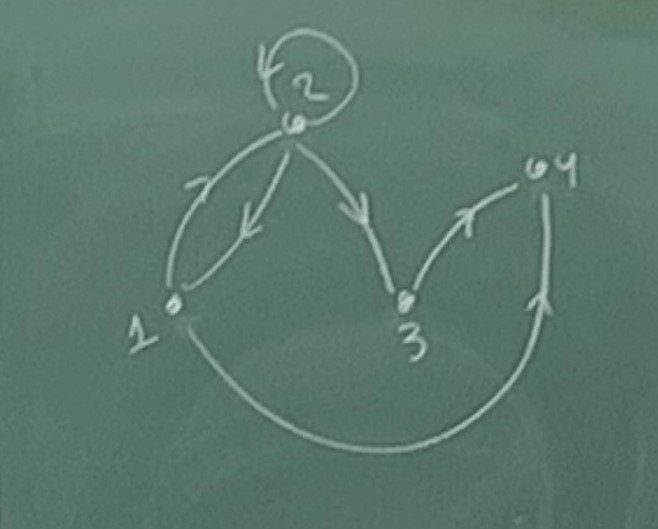
\includegraphics[scale=0.25]{imgs/lesson-21-11-23/img01-21-11-23.jpg}\\
        \end{figure}
        $A=\begin{pmatrix}
            0 & 1 & 0 & 1\\
            1 & 1 & 1 & 0\\
            0 & 0 & 0 & 1\\
            0 & 0 & 0 & 0
        \end{pmatrix}$\\
        \underline{Sats} Antalet riktade vägar i G av längd k frpn nod i till nod j ges av talet på plats (i,j) i matrisen\\
        $A^{k}=A A \ldots A$, k ggr, där A är grannmatrisen till G
    \clearpage
    \section{Talteori (kap 5)}
    Teorin flr heltalen $\mathbb{Z}$\\
    \underline{Första målet} Visa att varje positivit heltal kan skrivas som en produkt av primtal på ett unikt sätt.\\\\
    \underline{Delbarhet} Låt $a,b\in \mathbb{Z}$.\\
    Vi säger att \underline{a delar b} om det finns ett $m\in \mathbb{Z}$ så att $b=a\cdot m$.\\
    (Informellt a delar b om antingen $a=0=b$ eller $\frac{b}{a}$ är ett heltal)
    \\\\
    Skriver $a\mid b$ om a delar b, och $a\nmid b$ om inte delar b.\\\\
    \underline{\textbf{Ex}}\\
    $a\mid b$ ty $4=2\cdot 2$, $3\mid 2$ ty $12=3\cdot 4$\\
    $5\nmid 24$ då $5m\neq 24 \forall m\in \mathbb{Z}$\\
    $0\mid 0$ ty $0m=0 \forall m\in \mathbb{Z}$\\
    Delbarhet är en relation på $\mathbb{Z}$.\\
    \subsection{Några egenskaper (5.4 i boken)}
    \begin{enumerate}
        \item $a\mid 0 \forall a\in \mathbb{Z}$
        \item $a\mid a \forall a\in \mathbb{Z}$ (reflexivitet)
        \item $a\mid b\wedge b\mid c \Rightarrow a\mid c \forall a,b,c\in \mathbb{Z}$ (transivitet)
        \item $0\nmid a$ om $a\neq 0$
        \item Låt $a,b,c\in \mathbb{Z}$. Då gäller $(a\mid b\wedge a\mid c)\Leftrightarrow (a\mid xb+yc \forall x,y\in \mathbb{Z})$
    \end{enumerate}
    \underline{Bevis av 5)}\\
    $\Leftarrow$ : Antag att $a\mid xb+yc$ oavsett vad x och y är ($x,y\in \mathbb{Z}$)\\
    Om $x=1$ och $y=0$, så får jag $a\mid 1\cdot b+0\cdot c=b$, dvs $a\mid b$.\\
    Om $x=0$ och $y=1$, så får jag $a\mid 0\cdot b+1\cdot c=c$, dvs $a\mid c$.\\
    Så $a\mid b\wedge a\mid c$.\\\\
    $\Rightarrow$ : Antag att $a\mid b$ och $a\mid c$, så $\exists m,n\in \mathbb{Z}$ så att $b=a\cdot m$ och $c=a\cdot n$.\\
    Om $x,y\in \mathbb{Z}$ så är\\
    \indent $xb+yc=xam+yan=a(xm+yn)\Rightarrow a\mid xb+yc$.\\
    \\
    Delbarhet är reflexiv, transitiv och "nästan asymmetrisk".

    \subsection{Sats 5.7}
    Om $a\mid b$ och $b\mid a$, då är antingen $a=b$ eller $a=-b$.
    \subsubsection{Bevis}
    \underline{Fall 1:} $a=0$: $a\mid b \Rightarrow b=0 \Rightarrow a=b=-b$.\\
    \underline{Fall 2:} $a\neq 0$: $a\mid b$ betyder $\exists m\in \mathbb{Z} : b=am$\\
    \indent $b\mid a$ betyder $\exists n\in \mathbb{Z} : a=bn$,\\
    så $a=bn=amn\Rightarrow 1=mn\Rightarrow m=n=1$ eller $m=n=-1$\\
    $m=n=1$ ger $a=bn=b$, $m=n=-1$ ger $a=bn=-b$ v.s.b

    \subsection{Division med rest}
    \underline{}{"Divisionsalgoritmen":}\\
    Låt $a\in \mathbb{Z}$, $b\in \mathbb{Z_{+}}$. Då finns unika $q,r\in \mathbb{Z}$ så att\\
    \indent $a=qb+r$, med $0\leq r<b$.\\
    q kallas för \underline{kvoten}, r kallas \underline{resten}\\\\
    \underline{\textbf{Ex}} $17=3\cdot 5+2$ som är skriven på formen $a=q\cdot b+r$\\
    \\
    q är det största heltalet så att $a-qb\geq 0$.\\
    Och r är då $a-qb$.

    \subsection{Gemensamma delare}
    \underline{Def:} $a,b\in \mathbb{Z}$, då varken a eller b är =0\\
    En \underline{Gemensam delare} till a och b är ett $d\in \mathbb{Z}$ så att $d\mid a$ och $d\mid b$.\\\\
    \underline{\textbf{Ex}}\\
    \indent 2 är en gemensam delare till 16 och 24\\
    \indent 1 är en gemsensam delare till a och b där $a,b\in \mathbb{Z}$\\
    \indent -7 är en gemensam delare till 28 och 49\\
    \indent 5 är inte en gemensam delare till 15 och 24\\\\
    
    En gemensam delare d till a och b uppfyller (om $a\neq 0$)
    \begin{itemize}
        \item $d\leq |a|$, så det finns alltid en störstagemensamma \underline{delare} till a och b
        \item Skrivs sgd(a,b) och är alltid positiv
    \end{itemize}
    \underline{\textbf{Ex}} a=4, b=6\\
    \indent 4 har positiva delare 1,2,4\\
    \indent 6 har positiva delare 1,2,3,6\\
    så de positiva gemensamma delarna är 1 och 2, och sgd(4,6)=2
    \\\\
    \underline{Def:} Om sgd(a,b)=1 säger vi att a och b är \underline{relativt prima}.\\
    \subsection{Sats (5.14)}
    \begin{enumerate}
        \item Om $a\in\mathbb{Z_{+}}$ så är sgd(a,0)=a.
        \item $\forall a,b,n\in \mathbb{Z}$ så är sgd(a+nb,b)=sgd(a,b)
    \end{enumerate}
    \subsubsection{Varför?}
    \begin{enumerate}
        \item $a\mid a$ och $a\mid 0$ så a är en gemensam delare till a och 0. Om $d\mid a$ så är $d\leq a$, så måste a vara största gemensamma delaren till a och 0.
        \item Visar att (a,b) och (a+nb,b) har exakt samma gemensamma delare. Då måste också sgd(a,b)=sgd(a+nb,b).\\
                Om $d\mid a$ och $a\mid b$, så måste också $d\mid a+nb$ enligt sats 5.4 (del 5).\\
                Om $d\mid a+nb$ och $d\mid b$, så måste också $d\mid (a+nb)-nb$, dvs $d\mid a$ v.s.b
    \end{enumerate}
    \subsection{Euklides algoritm}
    $a,b\in \mathbb{Z_{+}}$. $a\geq b$. Genom upprepad division med rest får vi\\
    \indent $a=bq_{1}+r_{1}$, $0\leq r_{1}<b$\\
    \indent $b=r_{1}q_{2}+r_{2}$, $0\leq r_{2}<r_{1}$\\
    \indent $r_{1}=r_{2}q_{3}+r_{3}$, $0\leq r_{3}<r_{2}$\\
    \indent \vdots\\
    \indent $r_{n-2}=r_{n-1}q_{n}+r_{n}$,\\
    \indent $r_{n-1}=r_{n}q_{n+1}+r_{n+1}$\\
    Slutar när resten är 0. Då är $sgd(a,b)=r_{n}$. (Sista resten som inte är 0)\\\\
    \underline{\textbf{Ex}}\\
    Hitta sgd(16,24)\\
    \indent $24=16\cdot 1 + 8$\\
    \indent $16=8\cdot 2$, så sgd(16,24)=8\\
    Hitta sgd(7,15)\\
    \indent $13=7\cdot 1+6$\\
    \indent $7=6\cdot 1+1$ så sgd(7,13)=1\\
    \indent $6=1\cdot 6$\\
    \subsubsection{Varför funkar Euklides algoritm?}
    Enligt sats 5.14 är $sgd(a,b)=sgd(a-q_{1}b,b)=sgd(r_{1},b)=sgd(r_{1},b-q_{2}r_{1})=sgd(r_{1},r_{2})=\ldots=sgd(r_{n-1},r_{n})=sgd(r_{n-1}-r_{n}q_{n+1},r_{n})=sgd(0,r_{n})=r_{n}$\\
    \\
    \underline{\textbf{Ex}} a=876, b=204\\
    \indent $876=204\cdot 4+60$
    \indent $60=24\cdot 2+12$
    \indent $24=12\cdot 2$
    \indent så sgd(876, 204)=12.
    \indent $204=60\cdot 3+24$

    \section{Aritmetikens fundamentalsats}
    Låt $m\geq 2$ vara ett heltal. Då kan m skrivas på ett unikt sätt som $m=p_{1}, \ldots , p{r}$, där $p_{1}, \ldots , p_{r}$ är primtal och $p_{1}\leq \ldots \leq p_{r}$.\\
    \underline{\textbf{Ex:}}\\
    \indent $36=2\cdot 2\cdot 3\cdot 3$
    \indent $10=2\cdot 5$\\
    \indent $17=17$
    \begin{tabbing}
        \underline{Bevis:}\=\\
        \>Först $n\leq ar$ vi att det finns en primtalsfaktorisering, med strak induktion:\\
        \>\underline{Basfall:}\=\\
        \>\>$m=2$, $2=2$ är ett primtal\\
        \>Induktionssteget:\\
        \>\>Säg att varje tal $k<m$ har en primtalsfaktorisering. 
        Om m är ett primtal är vi klara ($m=m$ är en primtalsfaktorisering).
        Om m är ett sammansatt tal, så är $m=ab$, med $1\leq a$, $1\leq b$ heltal.
        Då är $a,b<m$, så $a=p_{1}\cdot \ldots \cdot p_{s}$, $b=p_{s+1}$
    \end{tabbing}

    SKRIV UTIFRÅN BILDER
    \clearpage
    \section{Kongruenser}
    Idag är det tisdag. VIlken veckodag är det om:
    \begin{enumerate}
        \item 6 dagar? (Måndag)
        \item 10 dagar? (Fredag)
        \item 106 dagar? (Onsdag)
    \end{enumerate}
    Hur kan man räkna? Cykler av 7 dagar
    \begin{enumerate}
        \item $6$ dagar framåt = 1 dag bakåt -> Måndag
        \item $10=7+3$, 10 dagar framåt = 3 dagar framåt -> Fredag
        \item $106=7\cdot 15+1$, så 106 dagar framåt = 1 dag framåt -> Onsdag
    \end{enumerate}
    Matematiskt kan man ställa upp det så här:
    \indent Måndag-Söndag representerar vi med 1 till 7.\\
    \indent Tisdag = 2.
    \begin{enumerate}
        \item $2+6=8=7+1,$, 1 = Måndag
        \item $2+10=12=7+5$, 5 = Fredag
        \item $2+106=108=7\cdot 15+3$, 3 = Onsdag
    \end{enumerate}
    kallas \underline{restträkning modulo 7} eller \underline{kongruensräkning modulo 7}. 
    7 är "cyckel", kallas modulus.
    I andra exempel har man ett annat modulus, t.ex 12 eller 24.\\
    Rent matematiskt kan vi välja vilket heltal $n\in \mathbb{Z_{+}}$ som helst som modulus.
    Jag vill betrakta två hetlal som "samma" om deras differens är en multipel av n.\\\\
    \underline{Hur?} Ekvivalensrelation.\\
    \underline{Def:} Låt $n\in \mathbb{Z_{+}}$. 
    Vi definierar en relation "$a\equiv b$ modulo $n$" på $\mathbb{Z}$ om $n\mid a-b$ (dvs $a-b$ är en multipel av n)\\
    Utläses "a är kngruent med b modulo n". Skrivs oftast $a\equiv b$ mod $n$ eller $a\equiv b$ $(n)$\\
    \underline{\textbf{Ex:}}
    \begin{enumerate}
        \item Om $n=7$, så är $8\equiv 1$ $(7)$ eftersom $8-1=7$ är en multipel av 7.\\
            Också $108\equiv 3$ $(7)$, eftersom $108-3=105=7\cdot 15$ är en multipel av 7.
            Däremot är $11\/\nequiv 3$ $(7)$, eftersom $11-3=8$ inte är en multipel av 7
    \end{enumerate}
    \underline{Sats} Kongruens mod n är en kvivalensrelation.\\\\
    \underline{Bevis} Skall kolla att kongruens mod n är reflexiv, symmetrisk och transitiv.\\
    \indent \underline{Reflexiv} $a\equiv a$ mod $n$? ja, eftersom $a-a=0$, som är delbart med n\\
    \indent \underline{Symmetrisk} Om $a\equiv b$ mod $n$, 
    så gäller $n\mid a-b$, om $n\mid a-b$,
     \\\indent så $n\mid (-1)(a-b)=n\mid b-a$, dvs $b\equiv a$ mod $n$\\
    \indent \underline{Transitiv} Antag att $a\equiv b$ mod $n$ och $b\equiv c$ mod $n$, 
    dvs $n\mid a-b$ och $n\mid b-c$.
    \\\indent Då gäller $n\mid (a-b)+(b-c)=n\mid a-c$, dvs $a\equiv c$ mod $n$\\\\
    \subsection{Hur ser ekvivalensklasserna för kongruens mod n ut?}
    Låt $a\in \mathbb{Z}$.\\
    \indent $[a]=\{b\in\mathbb{Z}\mid b\equiv a$ mod $n\}$ är definitionen av en ekvivalensklass\\
    Enligt divisionsalgoritmen finns ett unikt $r\in \mathbb{Z}$ med $0\leq r\leq n-1$ så att $a=nq+r$ dvs $a\equiv r$ mod $n$\\
    $r\in [a]$, så $[a]=[r]=\{\ldots , r-2n, r-n, r, r+n, r+2n, \ldots\}$\\
    \underline{\textbf{Ex:}} $n=4$\\
    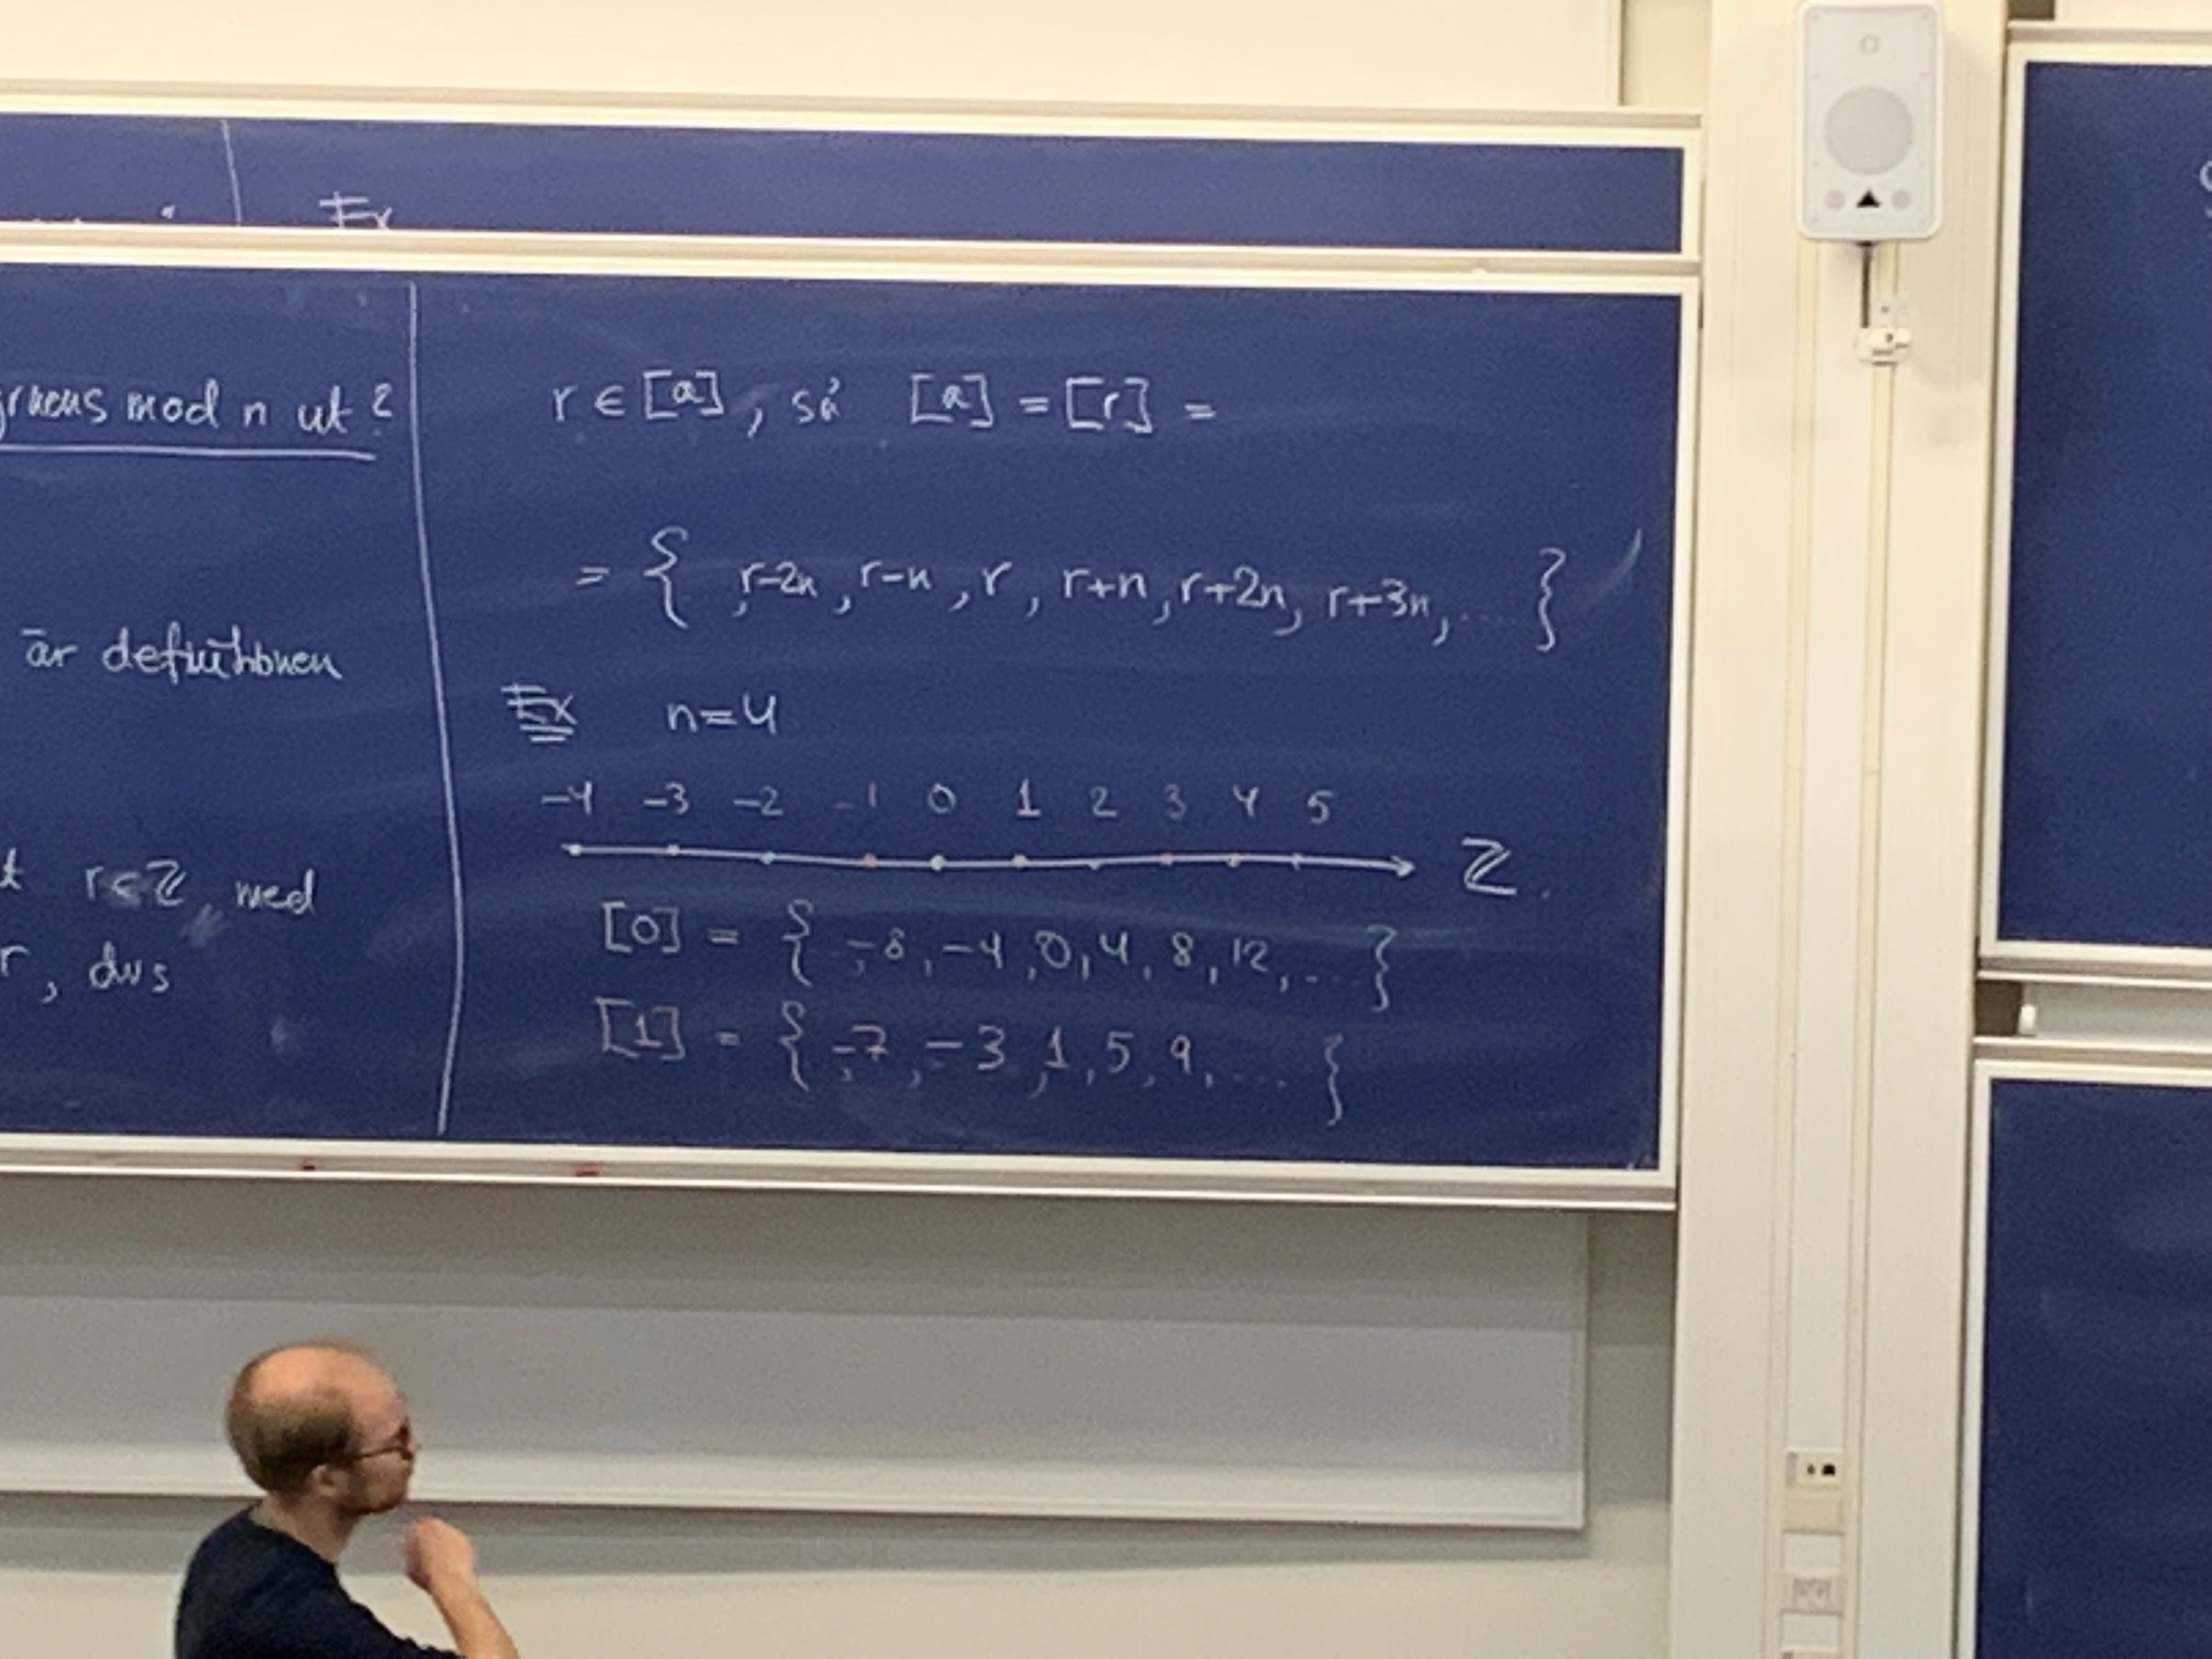
\includegraphics[scale=0.05]{imgs/lesson-21-12-07/img01-21-12-07.png}\\
    $[0]=\{\ldots, -8, -4, 0, 4, 8, \ldots\}$\\
    $[1]=\{\ldots, -7, -3, 1, 5, 9, \ldots\}$\\
    $[2]=\{\ldots, -6, -2, 2, 6, 10, \ldots\}$\\
    $[3]=\{\ldots, -5, -1, 3, 7, 11, \ldots\}$\\
    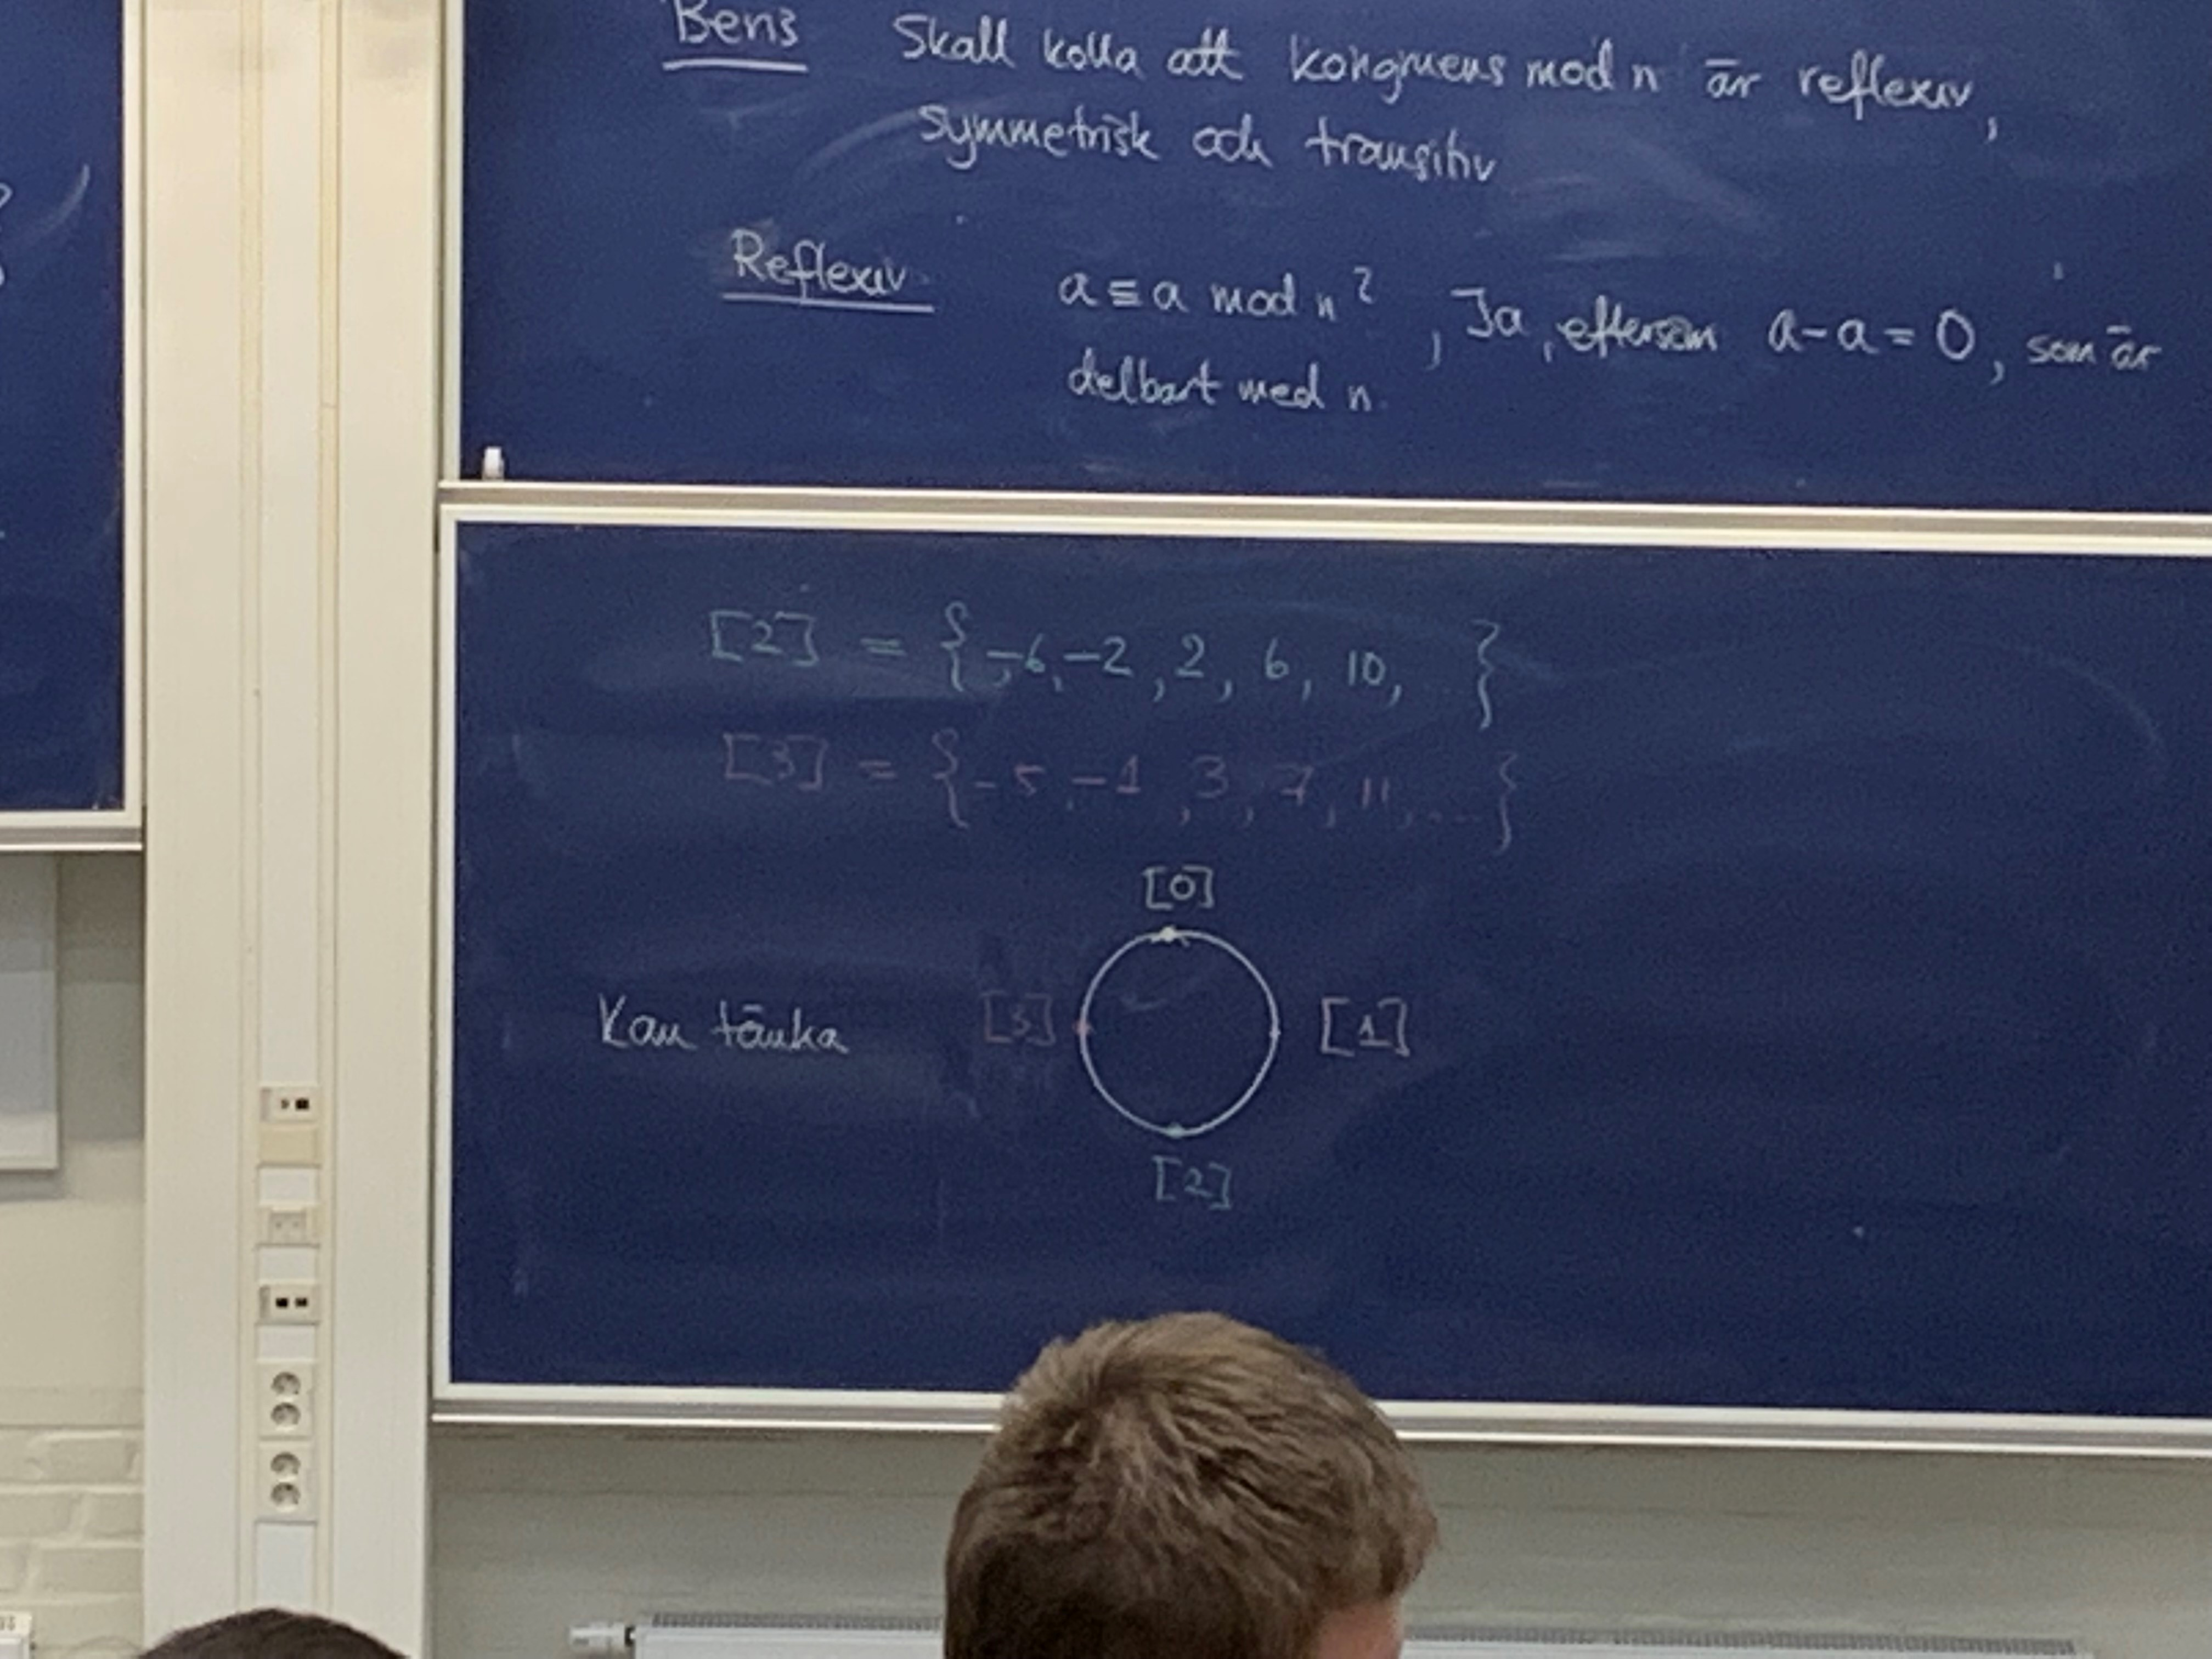
\includegraphics[scale=0.05]{imgs/lesson-21-12-07/img02-21-12-07.png}\\
    \subsection{Add, sub, multi och divi modulo n}
    Ekvivalensklasserna till relationen $\equiv$ mod n.\\
    Det finns n st olika \underline{kongruensklasser} modulo n:\\
    \indent $[0]_[n], [1]_[n], [2]_[n], \ldots, [n-1]_[n]$\\
    Ett tal $a\in \mathbb{Z}$ tillhör $[r]_{n}$, där r är resten vid division av a med n. (dvs $a=q\cdot n+r$, $+\leq r\leq n$)\\
    \underline{Def:} $\mathbb{Z_{n}}=\{[0]_[n], [1]_[n], \ldots, [n-1]_[n]\}$, mängden av alla kongruensklasser modulo n.
    \subsubsection{Addition, subtraktion och multiplikation}
    \underline{Sats (5.38)} $a,b,c,d\in \mathbb{Z}$, $n\in \mathbb{Z_{+}}$\\
    \indent Säg att $a\equiv c$ $(n)$ och $b\equiv d$ $(n)$. Då är 
    \begin{enumerate}
        \item $a+b\equiv c+d$
        \item $a-b\equiv c-d$
        \item $ab\equiv cd$
    \end{enumerate}
    \underline{\textbf{Ex:}} $6\cdot 9$ mod $7$?\\
    \indent $6\cdot 9=54=7\cdot 7+5\equiv 5$ $(7)$\\
    \indent $6\cdot 9\equiv (-1)\cdot 2\equiv -2\equiv 5$ $(7)$\\\\
    \underline{Varför är satsen sann?}\\
    \begin{enumerate}
        \item Vill visa $a+b\equiv c+d$ $(n)$, dvs $n\mid (a+b)-(c+d)$.\\
                Vet att $n\mid a-c$ ($=a\equiv c$ $(n)$) och $n\mid b-d$ ($b\equiv d$ $(n)$).\\
                $(a+b)-(c+d)=(a-c)+(b-d)$, så $n\mid (a+b)-(c+d)$.
        \item Görs på liknande sätt
        \item Görs på liknande sätt
    \end{enumerate}
    \underline{\textbf{Ex:}} Vilken veckodag är den 1 april 2022?\\
    Idag: Onsdag 8 december 2021.\\
    Dagar kvar . mod 7:\\
    $23+31+28+31+1\equiv 2+3+0+3+1\equiv 9\equiv 2$ $(7)$\\
    Så 1 april 2022 är en fredag.\\\\
    \underline{Def:} Vi definierar addition, subtraktion och multiplikation på $\mathbb{Z_{n}}$ genom\\
    $[a]_{n}+[b]_{n}=[a+b]_{n}$\\
    $[a]_{n}-[b]_{n}=[a-b]_{n}$\\
    $[a]_{n}\cdot [b]_{n}=[a\cdot b]_{n}$\\
    \underline{Varför är denna definitionen okej?}
    Säg att $[a]_{n}=[c]_{n}$ och $[b]_{n}=[d]_{n}$. Är då\\
    \begin{enumerate}
        \item $[a+b]_{n}=[c+d]_{n}$?
        \item $[a-b]_{n}=[c-d]_{n}$?
        \item $[a\cdot b]_{n}=[c\cdot d]_{n}$?
    \end{enumerate}
    $[a]_{n}=[c]_{n}\Leftrightarrow a\equiv c$ $(n)$ och $[b]_{n}=[d]_{n}\Leftrightarrow b\equiv d$ $(n)$\\
    \begin{enumerate}
        \item $\Leftrightarrow a+b\equiv c+d$ $(n)$
        \item $\Leftrightarrow a-b\equiv c-d$ $(n)$
        \item $\Leftrightarrow a\cdot b\equiv c\cdot d$ $(n)$
    \end{enumerate}
    Så definitionen är ok.\\\\
    \underline{\textbf{Ex:}} I $\mathbb{Z_{4}}$\\
    \indent $[3]_{4}+[2]_{4}=[3+2]_{4}=[5]_{4}=[1]_{4}$\\
    \indent $[1]_{4}-[3]_{4}=[1-3]_{4}=[-2]_{4}=[2]_{4}$\\
    \indent $[2]_{4}\cdot [2]_{4}=[4]_{4}=[0]_{4}$
    \subsection{Division i $\mathbb{Z_{n}}$}
    Division i $\mathbb{Z}$ - normalt är $\frac{a}{b}$ inte ett heltal även om a och b är heltal.\\
    Så det kommer inte funka att göra på samma sätt.\\
    $\frac{[1]_{3}}{[2]_{3}}=[\frac{1}{2}]_{3}$ ??? vad är $[\frac{1}{2}]_{3}$? (Finns inte)
    \subsubsection{Vad är division?}
    $a,b\in \mathbb{C}$ eller i $\mathbb{R}$.\\
    $\frac{b}{a}=\frac{1}{a}\cdot b$ Divison a = multiplikation med $\frac{1}{a}$
    \underline{Vad är $\frac{1}{a}$?} $\frac{1}{a}$ är ett tal x så $x\cdot a=1$\\
    \underline{Med andra ord} $\frac{1}{a}$ är lösningen (om den finns!) på $a\cdot x=1$.\\
    Om a=0 har $a\cdot x=1$ ingen lösninge - går inte att dela med $0$.\\\\
    I $\mathbb{Z_{n}}$ Givet $[a]_{n}\in \mathbb{{Z}_{n}}$, när kan vi lösa $[a]_{n}[x]_{n}=[1]_{n}$?\\
    \underline{\textbf{Ex:}} Kan jag lösa $[2]_{3}[x]_{3}=[1]_{3}$?\\
    Ja, $[x]_{3}=[2]_{3}$ är en lösning\\
    $[2]_{3}[2]_{3}=[4]_{3}=[1]_{3}$
    \subsubsection{Att lösa $[a]_{n}[x]_{n}=[1]_{n}$}
    Samma som $[ax-1]_{n}=[0]_{n}$, dvs $n\mid ax-1$, dvs $\exists y\in \mathbb{Z}$\\
    $ax-1=ny\Leftrightarrow ax-ny=1$ (vilket är en linjjär diofantiskekvation!)\\
    $ax-ny=1$ är lösbar $\Leftrightarrow sgd(a,n)\mid 1\Leftrightarrow sgd(a,n)=1$ och vi kan lösa den genom Euklides algoritm. 
    Vår formel för den allmänna lösningen till $ax-ny=1$ ger att x är unik modulo n.\\\\
    \underline{Modulo 3:} Om
    \begin{itemize}
        \item $a=0$ finns inget x
        \item $a=1$, $x\equiv 1$ $(3)$
        \item $a=2$, $x\equiv 2$ $(3)$
    \end{itemize}
    \underline{Modulo 5:} Om
    \begin{itemize}
        \item $a=0$ finns inget x
        \item $a=1$, $x\equiv 1$ $(5)$
        \item $a=2$, $x\equiv 3$ $(5)$ $2\cdot 3=6\equiv 1$ $(5)$
        \item $a=3$ $x\equiv 2$ $(5)$
        \item $a=4$ $x\equiv 4$ $(5)$\\
                $4\equiv -1$ $x\equiv -1$
    \end{itemize}
    \underline{Def:} Låt $[a]_{n}\in \mathbb{Z_{n}}$. Om $sgd(a,n)=1$ så finns ett unikt $[x]_{n}\in \mathbb{Z_{n}}$ så att $[a]_{n}[x]_{n}=[1]_{n}$\\
    $[x]_{n}$ kallas för \underline{inversen till $[a]_{n}$}\\
    Ett heltal x med egenskapen $ax\equiv 1$ $(n)$ kallas för en \underline{invers till a modulo n}. 
    Om a har en invers modulo n säger vi att a är \underline{inverterbar modulo n}.\\\\
    \underline{\textbf{Ex:}} 4 är inverterbar mod 9, eftersom $sgd(4,9)=1$. Hur hittar vi inversen till 4 mod 9?\\
    \indent \underline{Euklides algoritm:}\\
    \indent $9=4\cdot 2+1$\\
    \indent $4=1\cdot 4$\\
    \indent Balänges\\
    \indent $1=9-4\cdot 2$, ta det här mod 9\\
    \indent $1\equiv 0-4\cdot 2\equiv (-2)\cdot 4$ $(9)$\\
    Så $x=-2$ löser $4x\equiv 1$ $(9)$, dvs -2 är en invers till 4 mod 9
    \section{Linjära kongruens ekvationer}
    \underline{\textbf{Ex:}} Lös $4x\equiv 3$ mod 11.
    \indent \underline{En lösning:} Prova allt!\\
    \begin{comment}
    $\begin{matrix}
        x & 
        0 & 
        1 & 
        2 & 
        3 & 
        4 & 
        5 & 
        6 & 
        7 & 
        8 & 
        9 & 
        10 \\
        4x & 
        0 & 
        4 & 
        8 & 
        21\equiv 1 & 
        16\equiv 5 & 
        20\equiv 9 & 
        24\equiv 2 & 
        28\equiv 6 & 
        32\equiv 10 &
        36\equiv 3 & 
        40\equiv 7
    \end{matrix}$\\
\end{comment}
    \indent Där $x\equiv 9$ mod 9 är lösningen.\\\\
    \indent \underline{Mer systematiskt} $4x\equiv 3$ mod 11
    \indent Vill multiplicera ekvationen med inversen till 4 (om den finns) modulo 11,
    för att "få bort" 4:an.\\
    Hitta inversne till 4 mod 11:\\
    $11=4\cdot 2+3\\
    4=3\cdot 1+1\\
    1=4-3=4-(11-4\cdot 2)=3\cdot 4-11\\
    1=3\cdot 4-11$ ger att $1\equiv 3\cdot 4$ mod 11.\\\\
    För en vanlig ekvation $4x=3$ hade vi delat med 4, dvs multiplicerat med $\frac{1}{4}$, dvs multiplicerat med inversen till 4.

    \section{Eulers $\Phi$-funktion}
    $n\in \mathbb{Z_{+}}$. $u(n)\{[x]_{n}\in \mathbb{Z_{n}} \mid [x]_{n}$ är inverterbar $\}=\{[x_{n}\in \mathbb{Z_{n}}]\mid sgd(x,b)=1\}\subseteq \mathbb{Z_{n}}$\\
    \underline{Def:} $\Phi (n) = \mid u(n) \mid$, dvs\\
    \indent $\Phi (n)=$ antalet tal i $\{1, \ldots, n\}$ som är relativt prima med n.\\\\
    \underline{\textbf{Ex:}}\\
    $\Phi (1) = 1$ $u(1)=\{1\}$\\
    $\Phi (2) = 1$ $\mathbb{Z_{2}}=\{[0]_{2}, [1]_{2}\}$ och $u(2)=\{[1]_{2}\}$ har ett element\\
    \underline{n=6}\indent $\mathbb{Z_{6}}=\{[0]_{6},[1]_{6},[2]_{6},[3]_{6},[4]_{6},[5]_{6}\}$\\
    \indent $u(6)=\{[1]_{6}, [5]_{6}\}$, så $\Phi (6)=2$.
    \subsection{Eulers sats}
    Om sgd(a,n)=1, så är $a^{\Phi (n)}\equiv 1$ $(n)$.\\
    För att vara användbar behöver man kunnaa beräkna $\Phi (n)$.\\\\
    \underline{p primtal} $\Phi (p^{k})=p^{k}-p^{k-1}=p^{k-1}(p-1)$. ($k\in \mathbb{Z_{+}}$)\\
    \underline{Varför?} Vill beräkna antalet a mellan 1 och $p^{k}$ som är relativt prima med $p^{k}$, dvs $sgd(a,p^{k})=1\Leftrightarrow p \not \mid a$\\
    \indent De a mellan 1 och $p^{k}$ med $p\mid a$ är $p,2p,3p,\ldots,p^{k}=p^{k-1}p^{k}$, så de är $p^{k-1}$ st\\
    Så antalet a med $p\not \mid a$ är $p^{k}-p^{k-1}$, så $\Phi (p^{k})=p^{k}-p^{k-1}$.\\\\
    \underline{Sats} (5.54) Om sgd(m,n)=1, så är $\Phi (m,n)=\Phi (m) \cdot \Phi (n)$.\\
    \underline{Varför?}\\
    $\Phi (mn)=$ antalet a mellan 0 och $mn-1$ som är relativt prima med mn.\\
    Definiera en funktion $\{0,1,\ldots,mn-1\}\rightarrow\{0,1,\ldots,m-1\}\times \{0,1,\ldots, n-1\}$ på följande sätt. \\
    Om $a\in\{0,1,\ldots,mn-1\}$ så är \indent $a=mq_{1}+r_{1}$\indent $r_{1}\in\{0,1,\ldots,m-1\}$\\
    \indent \indent \indent \indent \indent \indent \indent \indent \indent \indent $a=nq{2}+r_{2}$\indent $r_{2}\in\{0,1,\ldots,n-1\}$\\
    Vi sätter $f(a)=(r_{1},r_{2})$.
    \begin{enumerate}
        \item f är ingektiv: Om $f(a)=f(b)$, så är $a\equiv b$ $(m)$ och $a\equiv b$ $(n)\Rightarrow a\equiv b$ $(mn)$ enligt kinesiska restsatsen, så $a=b$ eftersom $a,b\in\{0,1,\ldots,mn-1\}$.
        \item Säg att $f(a)=(r_{1}, r_{2})$. Då är $sgd(a,mn)=1\Leftrightarrow sgd(r_{1},m)=1$ och $sgd(r_{2}, n)=1$
    \end{enumerate}
    \underline{Varför?} $sgd(a,mn)=1\Leftrightarrow sgd(a,mn)=1$ och $sgd(a,n)=1\Leftrightarrow sgd(r_{1},m)=1$ och $sgd(r_{2},n)=1$. (Jämför med motiveringen till varför Euklides algoritm fungerar)\\\\
    \underline{Alltså} f ger en bijektion mellan $\{a\mid a\in\{0,1,\ldots,mn-1\},sgd(a,mn)=1\}$ (har $\Phi (mn)$ element)
     och $\{x\mid x\in\{0,1,\ldots,mn-1\},sgd(x,m)=1\}\times \{y\mid y\in\{0,1,\ldots,n-1\},sgd(y,n)=1\}$. 
     Så $\Phi (mn)=\Phi (m)\Phi (n)$ v.s.b\\\\
     Om $n=p^{e_{1}}_{1}\ldots p_{r}^{e_{r}}$, med $p_{i}$ olika primtal och $e_{i}\geq 1$, så är $\Phi (n)=\Phi (p_{1}^{e_{1}}\ldots p_{r}^{e_{r}})=\Phi (p_{1}^{e_{1}})\ldots \Phi (p_{r}^{e_{r}})=(p_{1}^{e_{r}}-p_{1}^{e_{1}-1})\ldots (p_{r}^{e_{r}}-p_{r}^{e_{1}-1})$\\
     \underline{\textbf{Ex:}} $\Phi (6)= \Phi (2\cdot 3)=\Phi (2) \cdot \Phi (3)=(2^{1}-2^{0})(3^{1}3^{0})=(2-1)(3-1)=1\cdot 2=2$\\
     $\Phi (48)=\Phi (2^{4}\cdot 3)=\Phi (2^{4})\Phi (3)=(2^{4}-2^{3})(3^{1}-3^{0})=(16-8)(3-1)=8\cdot 2=16$\\\\
    \underline{Specialfall av Eulers sats} p primtal.
    \begin{enumerate}
        \item Om $p\not \mid a$, så är $a^{p-1}\equiv 1$ $(p)$.
        \item $a^{p}\equiv a$ $(p)$ för alla $a\in \mathbb{Z}$
    \end{enumerate}
    \underline{\textbf{Ex:}} Vilken entalssiffra har $3^{8}\cdot 77+2^{10}\cdot 121$?\\
    \indent Entalssiffra = rest vid division med 10
    $77\equiv 7$ $(10)$, $121\equiv 1$ $(10)$.\\
    $3^{8}$ $\Phi (10)=\Phi (2)\Phi (5)=1\cdot 4=4$, så $3^{8}=(3^{4})^{2}\equiv 1^{2}\equiv 1$ $(10)$\\
    $2^{10}$ kan inte använda Eulers sats då $sgd(2,10)=2\not =1$.\\
    $2^{8}\equiv -2$ $(10)$ så $2^{10}=2^{3\cdot 3+1}=(2^{3})^{3}\cdot 2=-(-2)2\equiv 4$ $(10)$.\\
    $3^{8}\cdot 77+2^{10}\cdot 121\equiv 1\cdot 7+4\cdot 1\equiv 11\equiv 1$ $(10)$\\
    Så entalssiffran är 1.

\end{document}